\section{曲面的同调群}
\sourcepage{39--40}
若 $K$ 是有限复形，则链群 $C_p(K)$ 的秩有限，因而闭链群 $Z_p(K)$ 的秩也有限。于是 $H_p(K)$ 有限生成，可以应用阿贝尔群基本定理。按照经典术语，$H_p(K)$ 的 Betti 数和挠系数分别称为 $K$ 的 \textbf{$p$ 维 Betti 数}和 \textbf{$p$ 维挠系数}。第二章将证明，这些数是 $|K|$ 的拓扑不变量。

过去，不仅在拓扑学中，在代数学和其他数学领域中，人们也十分重视数值不变量。如今，数学家往往认为同调群是更重要的概念，更倾向于研究这些群的性质，而不是计算其数值不变量。不过，在许多情形下，具体计算同调群，即求出给定空间的 Betti 数与挠系数，仍然很重要。

单纯同调群的最大优点之一，正是这样的计算确实可行。第 1.12 节将证明：有限复形 $K$ 的同调群可以有效计算。这意味着存在求出 $K$ 的 Betti 数与挠系数的具体算法。

本节计算紧致曲面的 Betti 数与挠系数。所用技巧看上去可能有些笨拙，似乎是为特定问题临时设计的；事实上，它们对相当广泛的一类空间都有效。后面研究 CW 复形时，将重新讨论这些技巧，说明它们属于一种系统的同调计算方法。

为明确起见，先定义曲面的含义。

\entry{定义}{1.7.1}\textbf{曲面}（surface）是非空、连通、具有可数基的 Hausdorff 空间 $X$，使得 $X$ 的每个点都有一个与 $\R^2$ 的某个开子集同胚的邻域。

第 4.8 节将定义 $m$ 维流形。依照那里的定义，每个曲面都是二维流形；但由于这里还要求曲面连通且具有可数基，并非每个二维流形都是曲面。

\noindent\textbf{约定：}为简化记号，今后将省略边界算子 $\partial_p$ 的维数下标 $p$，依靠上下文区分所指的算子。

我们将计算环面、Klein 瓶以及其他几个曲面的同调。这些曲面都能通过对矩形 $L$ 的各边作适当等同而构造。因此，先证明关于 $L$ 本身的某些事实。

\entry{引理}{1.7.2}设 $L$ 为图 1.7.1 的复形，其底空间为矩形。用 $\Bd L$ 表示底空间为该矩形边界的复形。把 $L$ 的每个 $2$ 维单形 $\sigma_i$ 都沿逆时针方向定向，任意给各 $1$ 维单形定向。则：
\begin{enumerate}[label=(\arabic*)]
\item $L$ 的每条 $1$ 维闭链都同调于由 $\Bd L$ 承载的某条 $1$ 维闭链。
\item 若 $d$ 是 $L$ 的 $2$ 维链，且 $\partial d$ 由 $\Bd L$ 承载，则 $d$ 是链 $\sum\sigma_i$ 的某个整数倍。
\end{enumerate}
\begin{center}
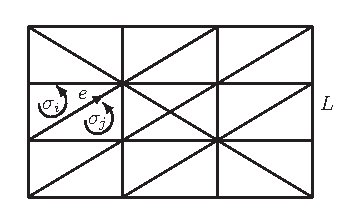
\includegraphics[width=64mm]{figures/1-7-1.pdf}\\图 1.7.1
\end{center}
\noindent\textbf{证明：}(2) 很容易。若 $\sigma_i,\sigma_j$ 有公共边 $e$，则 $\partial d$ 在 $e$ 上的值必须为 $0$。所以 $d$ 在 $\sigma_i$ 与 $\sigma_j$ 上的值相同。不断继续，可知 $d$ 在每个定向 $2$ 维单形上的值都相同。

为证明 (1)，采用例 1.6.13 的方法。给定 $L$ 的 $1$ 维链 $c$，逐步将它从各 $1$ 维单形上推开。先证明 $c$ 同调于由图 1.7.2 的子复形承载的链 $c_1$，再证明 $c_1$ 同调于由图 1.7.3 的子复形承载的链 $c_2$。最后，若原来的 $c$ 为闭链，则 $c_2$ 也为闭链。因此 $c_2$ 必须由 $\Bd L$ 承载，否则它在顶点 $v_1,\ldots,v_5$ 中至少一个上具有非零系数。\translatornote{原文说 $c_2$ 在顶点上有非零系数，按链的维数与论证，应为 $\partial c_2$ 在这些顶点上有非零系数。}\hfill$\square$
\begin{center}
\begin{minipage}{.48\textwidth}\centering
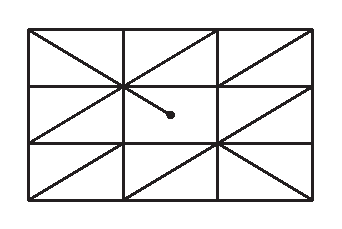
\includegraphics[width=62mm]{figures/1-7-2.pdf}\\图 1.7.2
\end{minipage}\hfill
\begin{minipage}{.48\textwidth}\centering
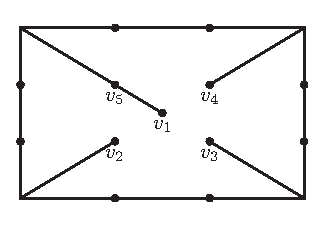
\includegraphics[width=60mm]{figures/1-7-3.pdf}\\图 1.7.3
\end{minipage}
\end{center}

\sourcepage{41--42}
\entry{定理}{1.7.3}设 $T$ 为图 1.7.4 的带标记矩形 $L$ 表示的复形，其底空间为环面。则
\[
H_1(T)\cong\Z\oplus\Z,\qquad H_2(T)\cong\Z.
\]
将 $L$ 的每个 $2$ 维单形沿逆时针方向定向，并用诱导的定向给 $T$ 的各 $2$ 维单形定向，以 $\gamma$ 表示它们的和。令
\[
\begin{aligned}
w_1&=[a,b]+[b,c]+[c,a],\\
z_1&=[a,d]+[d,e]+[e,a].
\end{aligned}
\]
则 $\gamma$ 生成 $H_2(T)$，而 $w_1,z_1$ 代表 $H_1(T)$ 的一组基。
\begin{center}
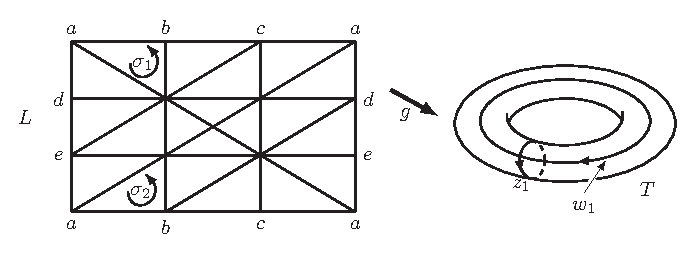
\includegraphics[width=119mm]{figures/1-7-4.pdf}\\图 1.7.4
\end{center}
\noindent\textbf{证明：}设 $g:|L|\to|T|$ 为粘合映射，$A=g(|\Bd L|)$。则 $A$ 同胚于两个只有一个公共点的圆周的并，这种空间称为\textbf{两个圆周的楔和}（wedge）。任意给 $T$ 的各 $1$ 维单形定向。因为 $g$ 只在 $\Bd L$ 的单形之间进行等同，引理 1.7.2 的论证可原样用于证明：
\begin{enumerate}[label=(\arabic*)]
\item $T$ 的每条 $1$ 维闭链都同调于由 $A$ 承载的 $1$ 维闭链。
\item 若 $d$ 为 $T$ 的 $2$ 维链，且 $\partial d$ 由 $A$ 承载，则 $d$ 是 $\gamma$ 的整数倍。
\end{enumerate}
另外，$T$ 中还有：
\begin{enumerate}[label=(\arabic*),start=3]
\item 若 $c$ 为由 $A$ 承载的 $1$ 维闭链，则 $c$ 形如 $nw_1+mz_1$。
\item $\partial\gamma=0$。
\end{enumerate}
由于 $A$ 就是图 1.7.5 的一维复形，(3) 很容易证明。(4) 也很直接：显然，$\partial\gamma$ 在所有不属于 $A$ 的 $1$ 维单形上都取值 $0$。直接检验可知，它在属于 $A$ 的每个 $1$ 维单形上也取值 $0$。例如，初等链 $[a,b]$ 在 $\partial\sigma_1$ 中的系数为 $-1$，在 $\partial\sigma_2$ 中的系数为 $+1$，所以 $\partial\gamma$ 在 $[a,b]$ 上取值 $0$，见图 1.7.4。$w_1,z_1$ 中其他定向 $1$ 维单形也有类似结论。
\begin{center}
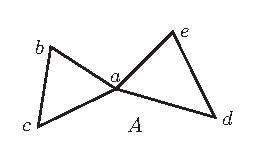
\includegraphics[width=48mm]{figures/1-7-5.pdf}\\图 1.7.5
\end{center}
利用 (1)--(4) 即可计算 $T$ 的同调。由 (1) 和 (3)，每条 $1$ 维闭链都同调于形如 $nw_1+mz_1$ 的闭链。这种闭链只有为零时才是边界：若 $c=\partial d$，由 (2) 得 $d=q\gamma$，再由 (4) 得 $c=\partial d=0$。所以 $H_1(T)\cong\Z\oplus\Z$，闭链 $w_1,z_1$ 的陪集构成一维同调的一组基。

为计算 $H_2(T)$，注意由 (2)，每条 $2$ 维闭链 $d$ 必定形如 $q\gamma$；由 (4)，每条这样的 $2$ 维链确为闭链，而且没有 $3$ 维链能以它为边界。所以 $H_2(T)\cong\Z$，由 $2$ 维闭链 $\gamma$ 生成。\hfill$\square$

\sourcepage{43--44}
\entry{定理}{1.7.4}设 $S$ 为图 1.7.6 的带标记矩形表示的复形，其底空间为 Klein 瓶。则
\[
H_1(S)\cong\Z\oplus\Z/2,\qquad H_2(S)=0.
\]
$H_1(S)$ 的挠元素由链 $z_1$ 代表，而将挠子群除去后的群的一个生成元由 $w_1$ 代表，其中
\[
w_1=[a,b]+[b,c]+[c,a],\qquad z_1=[a,d]+[d,e]+[e,a].
\]
\begin{center}
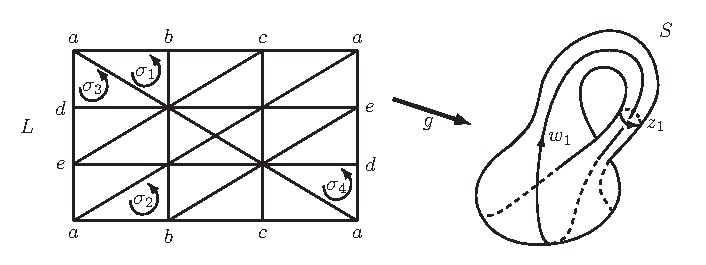
\includegraphics[width=121mm]{figures/1-7-6.pdf}\\图 1.7.6
\end{center}
\noindent\textbf{证明：}与定理 1.7.3 一样，令 $g:|L|\to|S|$ 为粘合映射，$A=g(|\Bd L|)$。$A$ 仍是两个圆周的楔和。将 $S$ 的各 $2$ 维单形沿逆时针方向定向，令其和为 $\gamma$；任意给各 $1$ 维单形定向。定理 1.7.3 证明中的 (1)、(2) 仍成立，因为它们不涉及边界上的具体等同方式。因为 $A$ 为两个圆周的楔和，(3) 也成立。最后的 (4) 改为
\[
\text{(4)}\qquad\partial\gamma=2z_1.
\]
直接计算即可验证。例如，$[a,b]$ 在 $\partial\sigma_1$ 中的系数为 $-1$，在 $\partial\sigma_2$ 中为 $+1$；而 $[a,d]$ 在 $\partial\sigma_3$ 和 $\partial\sigma_4$ 中的系数都为 $+1$。$w_1,z_1$ 中其他定向边也有类似结论。

综合这些事实，由 (1)、(3)，$S$ 的每条 $1$ 维闭链都同调于形如 $nw_1+mz_1$ 的闭链。若 $c=\partial d$，由 (2) 得 $d=p\gamma$，由 (4) 得 $\partial d=2pz_1$。因此，$nw_1+mz_1$ 为边界，当且仅当 $m$ 为偶数且 $n=0$。所以 $H_1(S)\cong\Z\oplus\Z/2$。闭链 $z_1$ 代表挠元素，$w_1$ 代表无限循环群 $H_1(S)/T_1(S)$ 的一个生成元。

由 (2)，$S$ 的每条 $2$ 维闭链都形如 $p\gamma$；由 (4)，当 $p\ne0$ 时它不是闭链，故 $H_2(S)=0$。\hfill$\square$

\entry{定理}{1.7.5}设 $P^2$ 为图 1.7.7 的带标记矩形所指定的复形。由例 1.4.10，其底空间称为射影平面。则
\[
H_1(P^2)\cong\Z/2,\qquad H_2(P^2)=0.
\]
\begin{center}
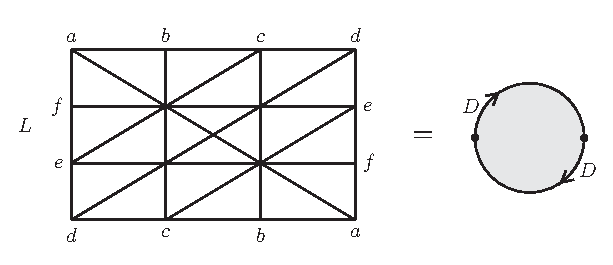
\includegraphics[width=107mm]{figures/1-7-7.pdf}\\图 1.7.7
\end{center}
\noindent\textbf{证明：}设 $g:|L|\to|P^2|$ 为粘合映射，$A=g(\Bd L)$，则 $A$ 同胚于圆周。与前两个定理一样定义 $\gamma$，令
\[
z_1=[a,b]+[b,c]+[c,d]+[d,e]+[e,f]+[f,a].
\]
定理 1.7.3 证明中的 (1)、(2) 仍成立。此外，容易验证：
\begin{enumerate}[label=(\arabic*),start=3]
\item 每条由 $A$ 承载的 $1$ 维闭链都是 $z_1$ 的整数倍。
\item $\partial\gamma=-2z_1$。
\end{enumerate}
于是 $H_1(P^2)\cong\Z/2$，$H_2(P^2)=0$。$H_1$ 的非零元素由闭链 $z_1$ 代表。\hfill$\square$

\sourcepage{45--46}
\entry{定义}{1.7.6}两个曲面 $S_1,S_2$ 的\textbf{连通和}（connected sum）定义为如下得到的曲面：从每个曲面中删去一个小开圆盘，再沿剩余部分的自由边界将它们粘合。记此空间为 $S_1\mathbin{\#}S_2$。

设 $T$ 为环面，空间 $T\mathbin{\#}T$ 称为\textbf{双环面}，如图 1.7.8。
\begin{center}
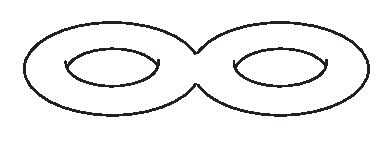
\includegraphics[width=69mm]{figures/1-7-8.pdf}\\图 1.7.8
\end{center}
空间 $P^2\mathbin{\#}P^2$ 可以表示为按图 1.7.9 所示方式粘合矩形各边所得到的商空间。注意，沿虚线 $C$ 剪开矩形，就得到图中所示的两个各自删去了一个开圆盘的射影平面。
\begin{center}
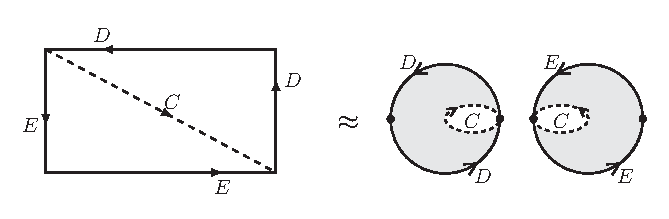
\includegraphics[width=116mm]{figures/1-7-9.pdf}\\图 1.7.9
\end{center}
\entry{定理}{1.7.7}设 $P^2\mathbin{\#}P^2$ 为两个射影平面的连通和。则
\[
H_1(P^2\mathbin{\#}P^2)\cong\Z\oplus\Z/2,\qquad
H_2(P^2\mathbin{\#}P^2)=0.
\]
\noindent\textbf{证明：}仍用前面的矩形 $L$ 表示 $P^2\mathbin{\#}P^2$，给顶点作与图 1.7.8 一致的标记。\translatornote{原文此处引用图 1.7.8，据粘合方式应为图 1.7.9。}此时复形 $A=g(|\Bd L|)$ 仍为两个圆周的楔和。令 $w_1$ 为沿矩形上边从右向左的 $1$ 维闭链，$z_1$ 为沿左边从上向下的 $1$ 维闭链，如图 1.7.9。定理 1.7.3 证明中的 (1)、(2) 仍成立，并且：
\begin{enumerate}[label=(\arabic*),start=3]
\item 每条由 $A$ 承载的 $1$ 维闭链都形如 $nw_1+mz_1$。
\item $\partial\gamma=2w_1+2z_1$。
\end{enumerate}
由此显然有 $H_2(P^2\mathbin{\#}P^2)=0$，但计算 $H_1$ 还需要进一步工作。

需要将以 $w_1,z_1$ 为基的群 $G$，对由 $2(w_1+z_1)$ 生成的子群 $H$ 取商。为此，要像自由阿贝尔群子群的基本定理 1.5.2 那样，为两群选择“相容”的基。此处容易看出，应使 $w_1+z_1$ 成为 $G$ 的一个基元素。确实可以做到：$\{w_1,w_1+z_1\}$ 与 $\{w_1,z_1\}$ 一样都是基，因为 $z_1=-w_1+(w_1+z_1)$，两组基可彼此表示。使用新基，便清楚地得到
\[
H_1(P^2\mathbin{\#}P^2)\cong\Z\oplus\Z/2.
\]
挠元素由 $w_1+z_1$ 代表，$w_1$ 代表 $H_1/T_1$ 的一个生成元。

注意，$w_1$ 不是唯一能代表 $H_1/T_1$ 的生成元的闭链。$z_1$ 也可以，因为 $\{z_1,w_1+z_1\}$ 是 $G$ 的一组基。同样，$\{2w_1+3z_1,w_1+z_1\}$ 也是基，因此 $2w_1+3z_1$ 也代表 $H_1/T_1$ 的一个生成元。事实上还有许多这样的闭链。\hfill$\square$

细心的读者可能注意到，这里的同调群与 Klein 瓶的同调群相同，见定理 1.7.4。这并非偶然，因为这两个空间实际上同胚，图 1.7.10 给出了证明示意。
\begin{center}
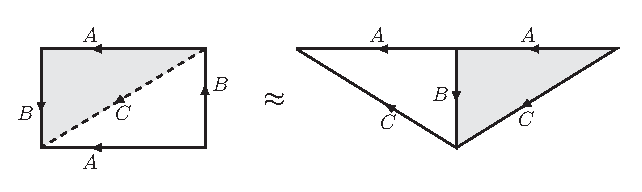
\includegraphics[width=113mm]{figures/1-7-10.pdf}\\图 1.7.10
\end{center}
\entry{定义}{1.7.8}图 1.7.11 所示的商空间称为\textbf{笨帽空间}（dunce cap）。
\begin{center}
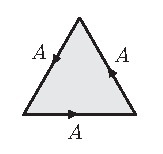
\includegraphics[width=31mm]{figures/1-7-11.pdf}\\图 1.7.11
\end{center}
习题 6 将推广笨帽空间。

下面的定理是十九世纪数学的一项重大成就。

\sourcepage{47--48}
\entry{定理}{1.7.9（紧致曲面分类定理）}每个紧致曲面都同胚于球面、$n$ 个环面的连通和，或 $m$ 个射影平面的连通和。

这里不证明此定理；可参阅 [Mun00] 第 12 章。

根据分类定理和已经算过的例子，你应当能够计算一般紧致曲面的同调群。此计算留作习题。

\subsection*{习题}
\begin{enumerate}
\item 设 $w_1,z_1$ 为图 1.7.6 中 Klein 瓶上的闭链。证明 $w_1+z_1$ 代表无限循环群 $H_1(S)/T_1(S)$ 的一个生成元。
\item 两个环面的连通和 $T\mathbin{\#}T$ 可表示为平面八边形区域的商空间，其中边界按图 1.7.12 等同。沿虚线分开八边形，就得到两个各自删去了开圆盘的环面。
\begin{enumerate}[label=(\alph*)]
\item 给图 1.7.13 中复形 $L$ 的顶点适当标记，构造底空间为 $T\mathbin{\#}T$ 的复形 $K$。
\item 仿照定理 1.7.3 计算 $T\mathbin{\#}T$ 的同调。具体地，令 $A$ 为 $\Bd L$ 在商映射下的像，则 $A$ 是四个圆周的楔和。将 $L$ 的每个 $2$ 维单形逆时针定向，令 $\gamma$ 为 $K$ 中相应定向单形的和。证明每条 $1$ 维闭链都同调于由 $A$ 承载的闭链；再证明每条边界由 $A$ 承载的 $2$ 维链都是 $\gamma$ 的整数倍。最后，分析由 $A$ 承载的 $1$ 维闭链，并计算 $\partial\gamma$，完成同调计算。
\end{enumerate}
\begin{center}
\begin{minipage}{.46\textwidth}\centering
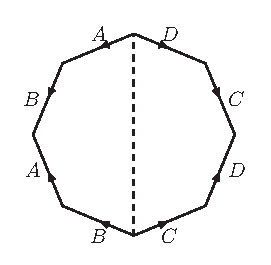
\includegraphics[width=49mm]{figures/1-7-12.pdf}\\图 1.7.12
\end{minipage}\hfill
\begin{minipage}{.46\textwidth}\centering
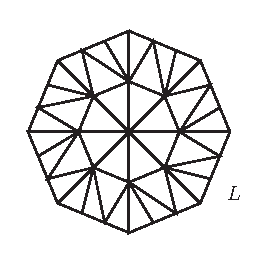
\includegraphics[width=47mm]{figures/1-7-13.pdf}\\图 1.7.13
\end{minipage}
\end{center}
\item 对图 1.7.12 中的复形 $L$ 作适当标记，表示四重连通和 $P^2\mathbin{\#}P^2\mathbin{\#}P^2\mathbin{\#}P^2$，并计算其一维、二维同调。\translatornote{原文引用图 1.7.12，但复形 $L$ 实际画在图 1.7.13。}
\item \begin{enumerate}[label=(\alph*)]
\item 定义 $n$ 个环面的连通和 $X_n=T\mathbin{\#}T\mathbin{\#}\cdots\mathbin{\#}T$，并计算一维、二维同调。
\item 定义 $n$ 个射影平面的连通和 $Y_n=P^2\mathbin{\#}\cdots\mathbin{\#}P^2$，并计算一维、二维同调。
\end{enumerate}
\item 计算 $T\mathbin{\#}P^2$ 的同调。它必同胚于习题 4 所列的哪个曲面？能否构造这个同胚？
\item \begin{enumerate}[label=(\alph*)]
\item 计算图 1.7.14 所示商空间的一维、二维同调。称此空间为“五重笨帽空间”。
\item 类似地定义“$k$ 重笨帽空间”，并计算其同调。
\end{enumerate}
\begin{center}
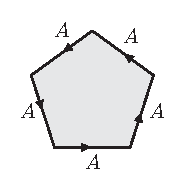
\includegraphics[width=35mm]{figures/1-7-14.pdf}\\图 1.7.14
\end{center}
\item 计算图 1.7.15 所示空间的同调。
\begin{center}
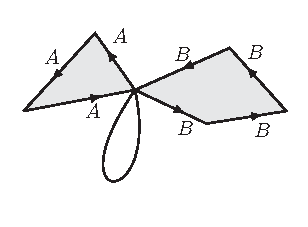
\includegraphics[width=58mm]{figures/1-7-15.pdf}\\图 1.7.15
\end{center}
\item 给定有限生成阿贝尔群 $G_1,G_2$，其中 $G_2$ 自由，证明存在有限二维复形 $K$，使 $|K|$ 连通，$H_1(K)\cong G_1$ 且 $H_2(K)\cong G_2$。
\end{enumerate}
